\section{Architektur}

Dieses Kapitel erläutert den Aufbau unserer Applikation.
Auf der Abbildung \ref{fig:overview} sind die wichtigsten Klassen und Interfaces der Applikation ersichtlich. In der Tabelle \ref{tab:class} sind
die wichtigsten Klassen beschrieben.

\begin{figure}[ht]
	\begin{center}
		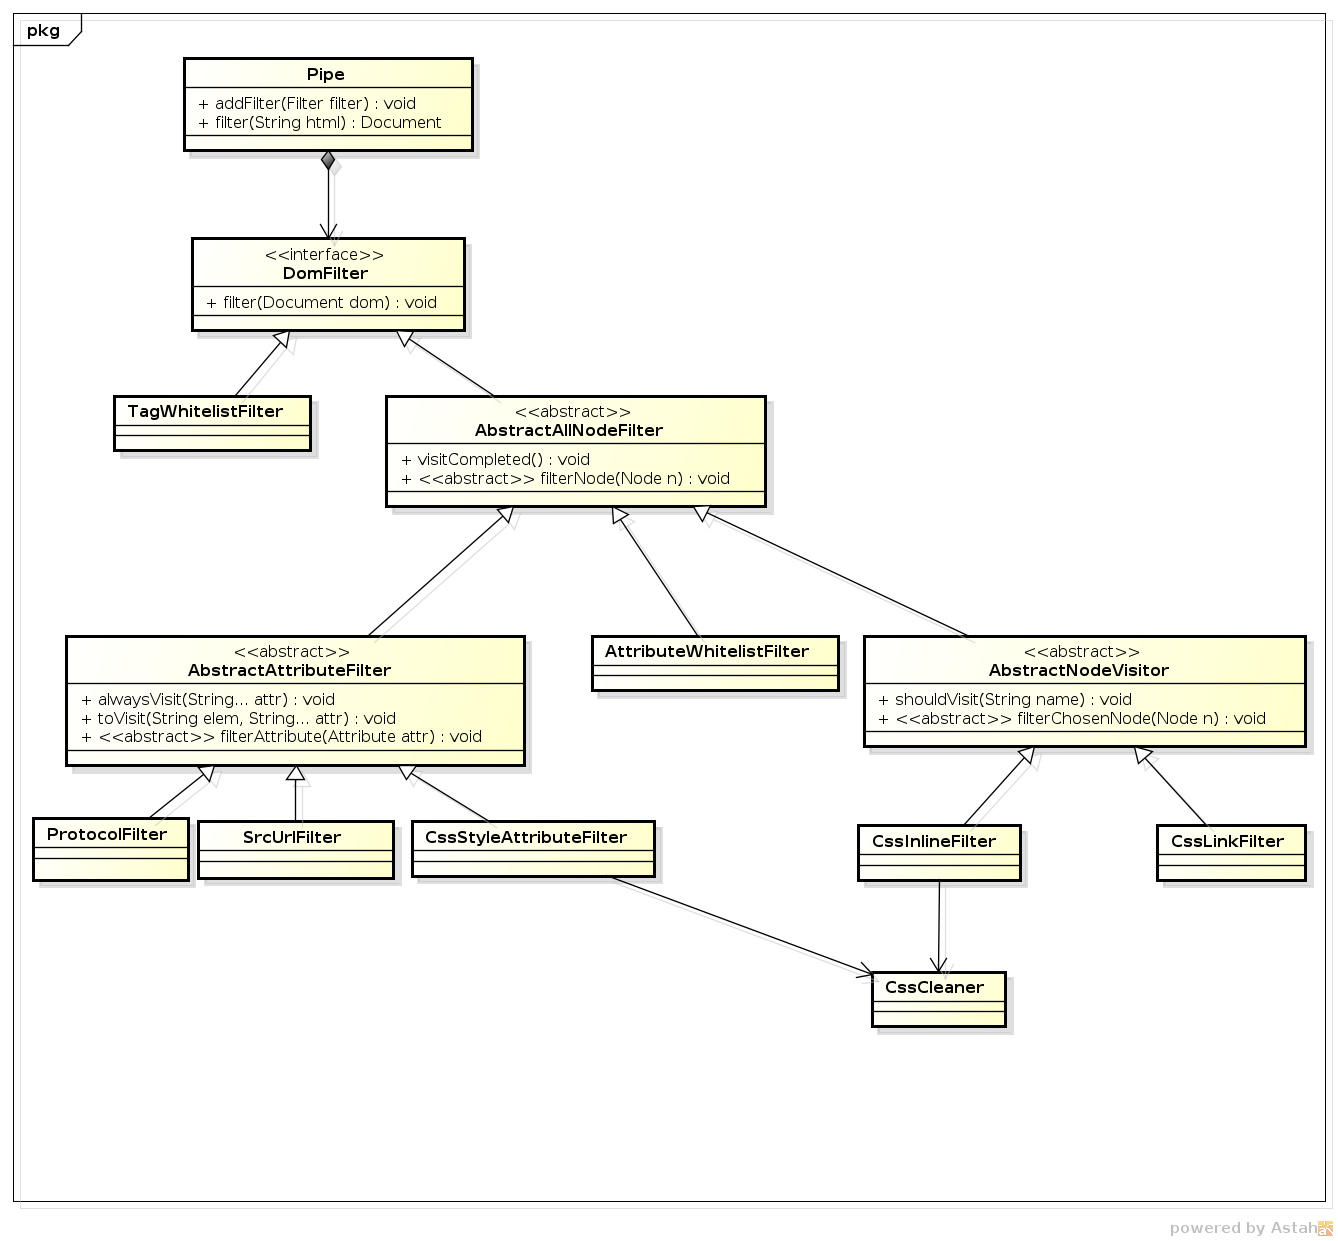
\includegraphics[width=1.0\textwidth]{./content/Class_Overview.png}
	\end{center}
	\caption{Übersicht über die Klassen und Interfaces}
	\label{fig:overview}
\end{figure}

\begin{table}[H]
\begin{center}
\begin{tabular}{l p{10.5cm} }
\hline
\textbf{Klasse} & \textbf{Beschreibung} \\ \hline \hline
Server      & Einstiegspunkt in die Applikation. Verwendet den Java HttpServer (com.sun.net.httpserver). Registiert die HttpHandler und startet den HttpServer. 
              Erstellt beim Start einen neuen User- und SessionManager. \\
XYHandler   & Nehmen HTTP Anfragen auf einer bestimmten URL entgegen und geben eine HTTP-Respone zurück. \\
UserManager & Verwaltet die Benutzer. Validiert beim Erstellen eines Benutzers den Benutzername und die E-Mail Adresse mit Hilfe der Klasse UserValidator.
              Wirft eine Exception, wenn der Benutzer nicht erstellt werden kann. \\
SessionManager & Verwaltet die ClientSessions. Ordnet jeder Session ein Token zu, mit welchem die Session identifiziert werden kann. \\
\hline \hline
\end{tabular}
\caption{Klassen}
\label{tab:class}
\end{center}
\end{table}

\begin{table}[H]
\begin{center}
\begin{tabular}{l l p{7cm} }
\hline
\textbf{Pfad} & \textbf{Handler}    & \textbf{Beschreibung} \\ \hline \hline
/             & WelcomeHandler          & Stellt die Loginseite index.html dar.\\
/register     & RegistrationHandler     & Verarbeitet die Registierungsanfrage und zeigt, wenn die Registierung erfoglreich war, einen Link zum Secure Content an. \\
/secured      & SecuredContentHandler   & Stellt wenn der Benutzer erfoglreich authentifiziert ist den Secure Content dar.\\
\hline \hline
\end{tabular}
\caption{URL-Mapping}
\label{tab:url-mapping}
\end{center}
\end{table}

\subsection{Authentifizierungsablauf}

Das Aktivitätsdiagramm Abbildung \ref{fig:process} beschreibt den Loginprozess bei einer HTTP-POST Anfrage auf /register mit einem gültigen Benutzernamen und E-Mail Adresse.
Als Resultat wird eine HTTP-Respone zurückgegeben, welche ein Cookie mit der Token ID setzt.

\begin{figure}[H]
	\begin{center}
		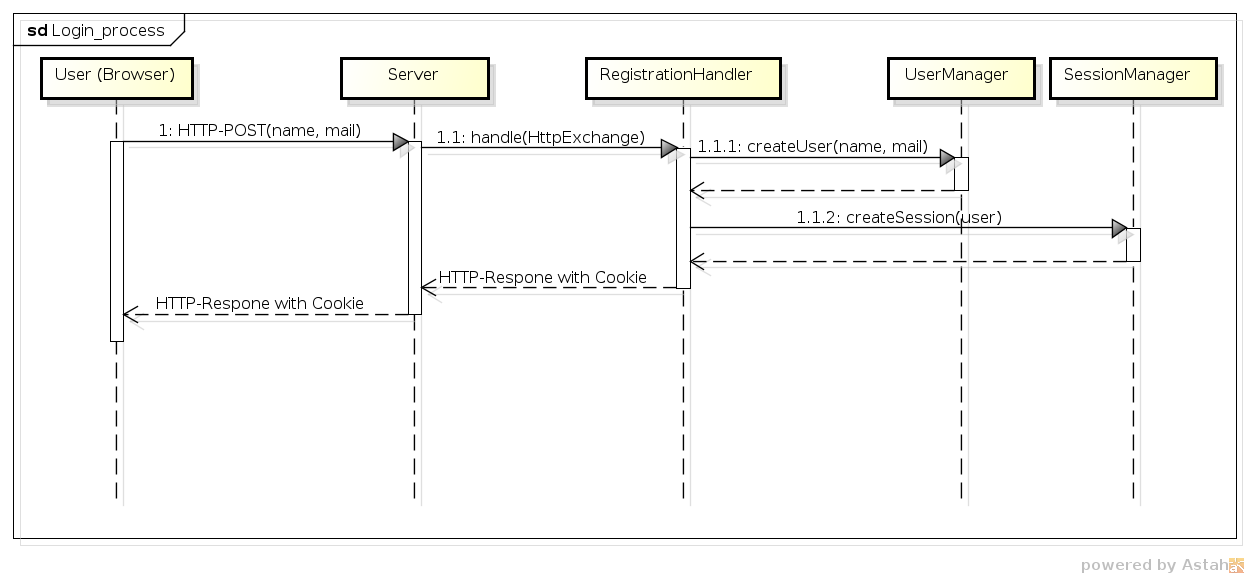
\includegraphics[width=1.0\textwidth]{./content/Login_process.png}
	\end{center}
	\caption{Loginprozess}
	\label{fig:process}
\end{figure}

\subsection{Cookie Authentification}

Die Schwierigkeit liegt darin, ein Cookie so aufzubauen, dass es für einen Angreifer schwierig ist (oder gar unmöglich), den Inhalt zu
erraten und so ein eigenes Cookie zu erstellen. Zu dem soll die Confidentiality der Daten, welche im Cookie gespeichert wurden
gewährleistet sin. Es soll also für einen angreifer nicht möglich sein, die Daten im Cookie zu lesen. Wir haben uns entschieden
ein \textit{Secure Cookie Protocol} zu implementieren, wie es in \cite{securecookie} beschrieben ist.

\subsubsection{Struktur}

Die innere Struktur des Cookie ist in Listing \ref{lst:cookie} beschrieben.

\begin{lstlisting}[caption=Innere Struktur des Cookie,label={lst:cookie}]
token | expiration timestamp | AES(data, k) 
| HMAC(tokent | expiration timestamp | data | SSL Session Key, k)

k = HMAC(token | expiration timestamp, sk)
sk = server key
HMAC(d,k) = Hash based message authentication code using data d and key k
\end{lstlisting}

\subsubsection{Verifizieren eines Cookies}

Das Listing \ref{lst:verify} zeigt den Ablauf des Verifizierens eines Cookies in pseudocode. 
Dies kann an mehreren Stellen fehlschlagen. Die dabei verwendete Funktion headerHash generiert 
aus einem Client Request Header einen hash, welcher den Client identifizieren soll. Das Verfahren
dazu wird in Listing{lst:header} beschrieben. Da im Cookie die IP des Clients sowie seine Header
als Hash gespeichert wurden, ist es für einen Angreifer extrem schwiereig ein gestohlenes Cookie
wiederzuverwenden. Er müsste es von der selben IP und mit dem exakt gleichen Header an den Server
schicken, was einen erfolgreichen Angriff extrem erschwert.
\newline
\begin{lstlisting}[caption=Verifikation eines Cookies,label={lst:verify}]
function checkCookie(cookie, requestHeader) {
    if(sessionmanager has no token = cookie.token) return FALSE
    sk = sessionmanager.getServerKeyForClient(cookie.token)

    if(cookie.expirationTime < current type) return FALSE

    k =  HMAC(token | expiration timestamp, sk)

    descypted = decrypt(cookie.data, k)

    if(decrypt failed) return FALSE

    expected = HMAC(tokent | expiration timestamp | data | SSL Session Key, k)

    if(expected != cookie.hash) return FALSE

    if(headerHash(request) != decrypted) return FALSE

    return TRUE
}
\end{lstlisting}
\newpage
\begin{lstlisting}[caption=Hashen des Headers eines Client Requests,label={lst:verify}]
function headerHash(request) {
    toHash = request.clientIP
    toHash += request.headers

    return SHA-256(toHash) 
}
\end{lstlisting}

\subsubsection{Erneuern eines Cookies}

Nach jedem Request eines Clients wird dessen Session Informationen und das dazugehörende Cookie
erneuert. So ist ein Cookie immer nur genau einmal gültig und kann von einem Angreifer so kaum 
benutzt werden. Das Verfahren ist in Listing \ref{lst:renew} erleutert. Dadurch, dass alle 
sessionrelevanten Informationen bei jedem Request komplett geändert werden, ändert sich die
Ausgangslage für einen Angreifer sehr schnell, was einen Angriff extrem erschwert.
\newline
\begin{lstlisting}[caption=Erneuern einer Session,label={lst:renew}]
function renewSession(oldTokent) {
    sess = getSession(oldToken)
    if(sess == null) return null

    removeSession(oldToken)

    newToken = generateToken()

    sess.expiringTime = current + TIMEOUT_TIME
    sess.currentKey = generateKey()
    sess.token = newToken

    putSession(newToken, sess)

    return newToken
}
\end{lstlisting}
